\documentclass{article}
\usepackage[utf8]{inputenc}
\usepackage{amsmath}
\usepackage{tikz}
\usetikzlibrary{positioning}

\title{Insertion Sort}
\author{Arvin Kushwaha}
\date{November 2021}

\begin{document}

\maketitle

\section{What is Insertion Sort?}

Insertion sort is an efficient technique for sorting small sequences. To describe the algorithm, I'll effectively reiterate the description provided in the textbook, "Introduction to Algorithms, 3e," which introduces it by means of imagining a set of playing cards (which I will render as just blocks of numbers (representing the associated value: Ace = 1, ..., King = 13), for LaTeX simplicity).

\begin{center}
    \begin{tabular}{|p{0.9\textwidth}|}
        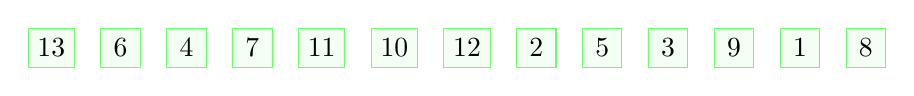
\begin{tikzpicture}[squarenode/.style={rectangle, draw=green!60, fill=green!5, thin, minimum size=5mm}]
        
        \node[squarenode] (1) {13};
        \node[squarenode] (2) [right=0.323cm of 1] {6};
        \node[squarenode] (3) [right=0.323cm of 2] {4};
        \node[squarenode] (4) [right=0.323cm of 3] {7};
        \node[squarenode] (5) [right=0.323cm of 4] {11};
        \node[squarenode] (6) [right=0.323cm of 5] {10};
        \node[squarenode] (7) [right=0.323cm of 6] {12};
        \node[squarenode] (8) [right=0.323cm of 7] {2};
        \node[squarenode] (9) [right=0.323cm of 8] {5};
        \node[squarenode] (10) [right=0.323cm of 9] {3};
        \node[squarenode] (11) [right=0.323cm of 10] {9};
        \node[squarenode] (12) [right=0.323cm of 11] {1};
        \node[squarenode] (13) [right=0.323cm of 12] {8};

        \end{tikzpicture}
    \end{tabular}
\end{center}

Imagine a set of shuffled diamond cards (pictured above), which we aim to sort from Ace to King. For \textbf{insertion sort}, we have a sequence of $n$ values, which we call \emph{keys}. These will be our card values. Now, let us reserve space for our new ordered set of cards.

\begin{center}
    \begin{tabular}{|p{0.9\textwidth}|}
        \begin{tikzpicture}[squarenode/.style={rectangle, draw=green!60, fill=green!5, thin, minimum size=5mm}]
        \end{tikzpicture}
    \end{tabular}
\end{center}

\begin{center}
    \begin{tabular}{|p{0.9\textwidth}|}
        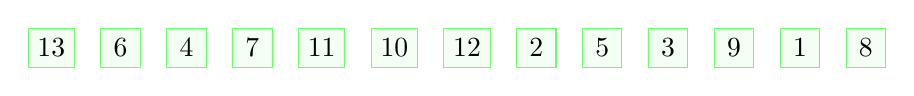
\begin{tikzpicture}[squarenode/.style={rectangle, draw=green!60, fill=green!5, thin, minimum size=5mm}]
        
        \node[squarenode] (1) {13};
        \node[squarenode] (2) [right=0.323cm of 1] {6};
        \node[squarenode] (3) [right=0.323cm of 2] {4};
        \node[squarenode] (4) [right=0.323cm of 3] {7};
        \node[squarenode] (5) [right=0.323cm of 4] {11};
        \node[squarenode] (6) [right=0.323cm of 5] {10};
        \node[squarenode] (7) [right=0.323cm of 6] {12};
        \node[squarenode] (8) [right=0.323cm of 7] {2};
        \node[squarenode] (9) [right=0.323cm of 8] {5};
        \node[squarenode] (10) [right=0.323cm of 9] {3};
        \node[squarenode] (11) [right=0.323cm of 10] {9};
        \node[squarenode] (12) [right=0.323cm of 11] {1};
        \node[squarenode] (13) [right=0.323cm of 12] {8};

        \end{tikzpicture}
    \end{tabular}
\end{center}

To perform \textbf{insertion sort}, we take cards one at a time from the unordered sequence and place it in the appropriate location in the to-be ordered sequence. To determine this appropriate location, we compare the card to each card already in the ordered sequence and insert it in the location where our card fails to be greater than the card in the ordered sequence it is being compared to. Let's do this for the first card!

\begin{center}
    \begin{tabular}{|p{0.9\textwidth}|}
        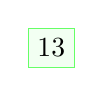
\begin{tikzpicture}[squarenode/.style={rectangle, draw=green!60, fill=green!5, thin, minimum size=5mm}]

        \node[squarenode] (1) {13};

        \end{tikzpicture}
    \end{tabular}
\end{center}

\begin{center}
    \begin{tabular}{|p{0.9\textwidth}|}
        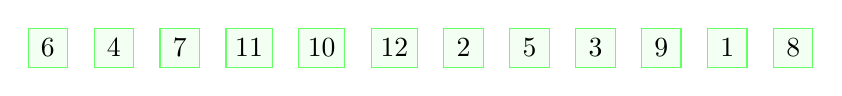
\begin{tikzpicture}[squarenode/.style={rectangle, draw=green!60, fill=green!5, thin, minimum size=5mm}]
        
        
        \node[squarenode] (2) {6};
        \node[squarenode] (3) [right=0.323cm of 2] {4};
        \node[squarenode] (4) [right=0.323cm of 3] {7};
        \node[squarenode] (5) [right=0.323cm of 4] {11};
        \node[squarenode] (6) [right=0.323cm of 5] {10};
        \node[squarenode] (7) [right=0.323cm of 6] {12};
        \node[squarenode] (8) [right=0.323cm of 7] {2};
        \node[squarenode] (9) [right=0.323cm of 8] {5};
        \node[squarenode] (10) [right=0.323cm of 9] {3};
        \node[squarenode] (11) [right=0.323cm of 10] {9};
        \node[squarenode] (12) [right=0.323cm of 11] {1};
        \node[squarenode] (13) [right=0.323cm of 12] {8};

        \end{tikzpicture}
    \end{tabular}
\end{center}

Well, that was rather lackluster, right? For the first value, its as simple as simply placing the card in the sequence, since we have no cards to compare the King (13) with.

Let's do the next card: 6. Well, first we have to compare 6 with 13. 6 is less than 13, so it gets placed right at the very beginning. How about 4? Well, comparing 4 to 6, we see that 4 is less than 6 and now 4 is our new first value. Here's our progress so far:

\begin{center}
    \begin{tabular}{|p{0.9\textwidth}|}
        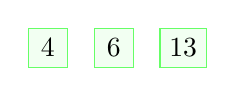
\begin{tikzpicture}[squarenode/.style={rectangle, draw=green!60, fill=green!5, thin, minimum size=5mm}]
            
        \node[squarenode] (1) {4};
        \node[squarenode] (2) [right=0.323cm of 1] {6};
        \node[squarenode] (3) [right=0.323cm of 2] {13};

        \end{tikzpicture}
    \end{tabular}
\end{center}

\begin{center}
    \begin{tabular}{|p{0.9\textwidth}|}
        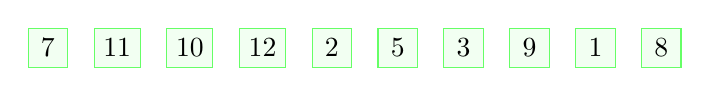
\begin{tikzpicture}[squarenode/.style={rectangle, draw=green!60, fill=green!5, thin, minimum size=5mm}]
        
        \node[squarenode] (4) {7};
        \node[squarenode] (5) [right=0.323cm of 4] {11};
        \node[squarenode] (6) [right=0.323cm of 5] {10};
        \node[squarenode] (7) [right=0.323cm of 6] {12};
        \node[squarenode] (8) [right=0.323cm of 7] {2};
        \node[squarenode] (9) [right=0.323cm of 8] {5};
        \node[squarenode] (10) [right=0.323cm of 9] {3};
        \node[squarenode] (11) [right=0.323cm of 10] {9};
        \node[squarenode] (12) [right=0.323cm of 11] {1};
        \node[squarenode] (13) [right=0.323cm of 12] {8};

        \end{tikzpicture}
    \end{tabular}
\end{center}

Finally, we've come to an interesting card: 7. Let's start the process again. Is 7 greater than 4? Yes? Okay, lets compare with 6. Is 7 greater than 6? Yes? Okay, now for 13. Since 7 is not greater than 13, we place it after 6 and before 13.

\begin{center}
    \begin{tabular}{|p{0.9\textwidth}|}
        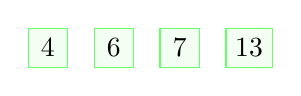
\begin{tikzpicture}[squarenode/.style={rectangle, draw=green!60, fill=green!5, thin, minimum size=5mm}]
            
        \node[squarenode] (1) {4};
        \node[squarenode] (2) [right=0.323cm of 1] {6};
        \node[squarenode] (3) [right=0.323cm of 2] {7};
        \node[squarenode] (4) [right=0.323cm of 3] {13};

        \end{tikzpicture}
    \end{tabular}
\end{center}

\begin{center}
    \begin{tabular}{|p{0.9\textwidth}|}
        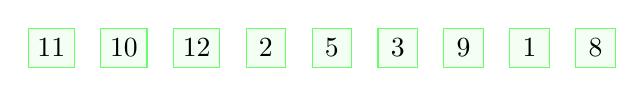
\begin{tikzpicture}[squarenode/.style={rectangle, draw=green!60, fill=green!5, thin, minimum size=5mm}]
        
        \node[squarenode] (5) {11};
        \node[squarenode] (6) [right=0.323cm of 5] {10};
        \node[squarenode] (7) [right=0.323cm of 6] {12};
        \node[squarenode] (8) [right=0.323cm of 7] {2};
        \node[squarenode] (9) [right=0.323cm of 8] {5};
        \node[squarenode] (10) [right=0.323cm of 9] {3};
        \node[squarenode] (11) [right=0.323cm of 10] {9};
        \node[squarenode] (12) [right=0.323cm of 11] {1};
        \node[squarenode] (13) [right=0.323cm of 12] {8};

        \end{tikzpicture}
    \end{tabular}
\end{center}

I think you get the gist of it by now. Lets quickly finish this up:

\begin{center}
    \begin{tabular}{|p{0.9\textwidth}|}
        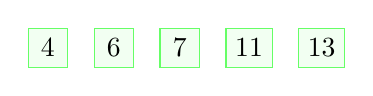
\begin{tikzpicture}[squarenode/.style={rectangle, draw=green!60, fill=green!5, thin, minimum size=5mm}]
            
        \node[squarenode] (1) {4};
        \node[squarenode] (2) [right=0.323cm of 1] {6};
        \node[squarenode] (3) [right=0.323cm of 2] {7};
        \node[squarenode] (4) [right=0.323cm of 3] {11};
        \node[squarenode] (5) [right=0.323cm of 4] {13};

        \end{tikzpicture}
    \end{tabular}
\end{center}

\begin{center}
    \begin{tabular}{|p{0.9\textwidth}|}
        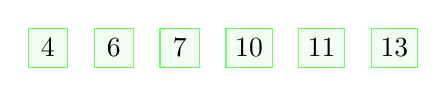
\begin{tikzpicture}[squarenode/.style={rectangle, draw=green!60, fill=green!5, thin, minimum size=5mm}]
            
        \node[squarenode] (1) {4};
        \node[squarenode] (2) [right=0.323cm of 1] {6};
        \node[squarenode] (3) [right=0.323cm of 2] {7};
        \node[squarenode] (4) [right=0.323cm of 3] {10};
        \node[squarenode] (5) [right=0.323cm of 4] {11};
        \node[squarenode] (6) [right=0.323cm of 5] {13};

        \end{tikzpicture}
    \end{tabular}
\end{center}

\begin{center}
    \begin{tabular}{|p{0.9\textwidth}|}
        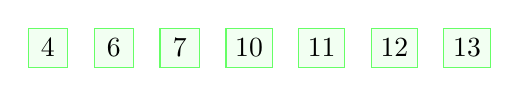
\begin{tikzpicture}[squarenode/.style={rectangle, draw=green!60, fill=green!5, thin, minimum size=5mm}]
            
        \node[squarenode] (1) {4};
        \node[squarenode] (2) [right=0.323cm of 1] {6};
        \node[squarenode] (3) [right=0.323cm of 2] {7};
        \node[squarenode] (4) [right=0.323cm of 3] {10};
        \node[squarenode] (5) [right=0.323cm of 4] {11};
        \node[squarenode] (6) [right=0.323cm of 5] {12};
        \node[squarenode] (7) [right=0.323cm of 6] {13};

        \end{tikzpicture}
    \end{tabular}
\end{center}

\begin{center}
    \begin{tabular}{|p{0.9\textwidth}|}
        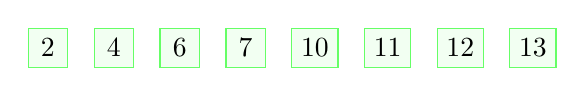
\begin{tikzpicture}[squarenode/.style={rectangle, draw=green!60, fill=green!5, thin, minimum size=5mm}]
        
        \node[squarenode] (1) {2};
        \node[squarenode] (2) [right=0.323cm of 1] {4};
        \node[squarenode] (3) [right=0.323cm of 2] {6};
        \node[squarenode] (4) [right=0.323cm of 3] {7};
        \node[squarenode] (5) [right=0.323cm of 4] {10};
        \node[squarenode] (6) [right=0.323cm of 5] {11};
        \node[squarenode] (7) [right=0.323cm of 6] {12};
        \node[squarenode] (8) [right=0.323cm of 7] {13};

        \end{tikzpicture}
    \end{tabular}
\end{center}

\begin{center}
    \begin{tabular}{|p{0.9\textwidth}|}
        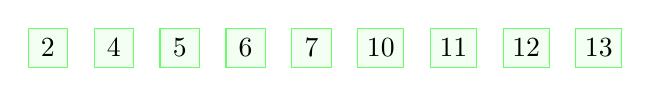
\begin{tikzpicture}[squarenode/.style={rectangle, draw=green!60, fill=green!5, thin, minimum size=5mm}]
        
        \node[squarenode] (1) {2};
        \node[squarenode] (2) [right=0.323cm of 1] {4};
        \node[squarenode] (3) [right=0.323cm of 2] {5};
        \node[squarenode] (4) [right=0.323cm of 3] {6};
        \node[squarenode] (5) [right=0.323cm of 4] {7};
        \node[squarenode] (6) [right=0.323cm of 5] {10};
        \node[squarenode] (7) [right=0.323cm of 6] {11};
        \node[squarenode] (8) [right=0.323cm of 7] {12};
        \node[squarenode] (9) [right=0.323cm of 8] {13};

        \end{tikzpicture}
    \end{tabular}
\end{center}

\begin{center}
    \begin{tabular}{|p{0.9\textwidth}|}
        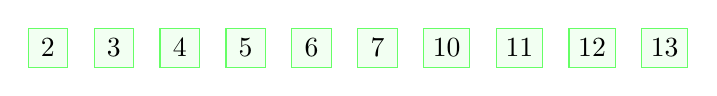
\begin{tikzpicture}[squarenode/.style={rectangle, draw=green!60, fill=green!5, thin, minimum size=5mm}]
        
        \node[squarenode] (1) {2};
        \node[squarenode] (2) [right=0.323cm of 1] {3};
        \node[squarenode] (3) [right=0.323cm of 2] {4};
        \node[squarenode] (4) [right=0.323cm of 3] {5};
        \node[squarenode] (5) [right=0.323cm of 4] {6};
        \node[squarenode] (6) [right=0.323cm of 5] {7};
        \node[squarenode] (7) [right=0.323cm of 6] {10};
        \node[squarenode] (8) [right=0.323cm of 7] {11};
        \node[squarenode] (9) [right=0.323cm of 8] {12};
        \node[squarenode] (10) [right=0.323cm of 9] {13};

        \end{tikzpicture}
    \end{tabular}
\end{center}

\begin{center}
    \begin{tabular}{|p{0.9\textwidth}|}
        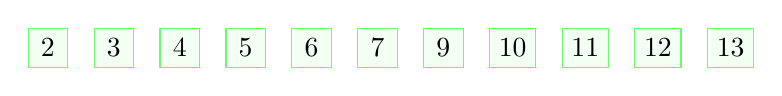
\begin{tikzpicture}[squarenode/.style={rectangle, draw=green!60, fill=green!5, thin, minimum size=5mm}]
        
        \node[squarenode] (1) {2};
        \node[squarenode] (2) [right=0.323cm of 1] {3};
        \node[squarenode] (3) [right=0.323cm of 2] {4};
        \node[squarenode] (4) [right=0.323cm of 3] {5};
        \node[squarenode] (5) [right=0.323cm of 4] {6};
        \node[squarenode] (6) [right=0.323cm of 5] {7};
        \node[squarenode] (7) [right=0.323cm of 6] {9};
        \node[squarenode] (8) [right=0.323cm of 7] {10};
        \node[squarenode] (9) [right=0.323cm of 8] {11};
        \node[squarenode] (10) [right=0.323cm of 9] {12};
        \node[squarenode] (11) [right=0.323cm of 10] {13};

        \end{tikzpicture}
    \end{tabular}
\end{center}

\begin{center}
    \begin{tabular}{|p{0.9\textwidth}|}
        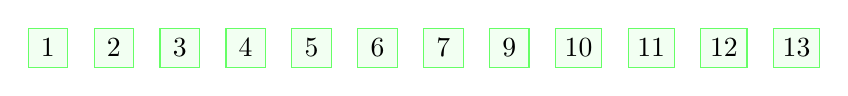
\begin{tikzpicture}[squarenode/.style={rectangle, draw=green!60, fill=green!5, thin, minimum size=5mm}]
        
        \node[squarenode] (1) {1};
        \node[squarenode] (2) [right=0.323cm of 1] {2};
        \node[squarenode] (3) [right=0.323cm of 2] {3};
        \node[squarenode] (4) [right=0.323cm of 3] {4};
        \node[squarenode] (5) [right=0.323cm of 4] {5};
        \node[squarenode] (6) [right=0.323cm of 5] {6};
        \node[squarenode] (7) [right=0.323cm of 6] {7};
        \node[squarenode] (8) [right=0.323cm of 7] {9};
        \node[squarenode] (9) [right=0.323cm of 8] {10};
        \node[squarenode] (10) [right=0.323cm of 9] {11};
        \node[squarenode] (11) [right=0.323cm of 10] {12};
        \node[squarenode] (12) [right=0.323cm of 11] {13};

        \end{tikzpicture}
    \end{tabular}
\end{center}

\begin{center}
    \begin{tabular}{|p{0.9\textwidth}|}
        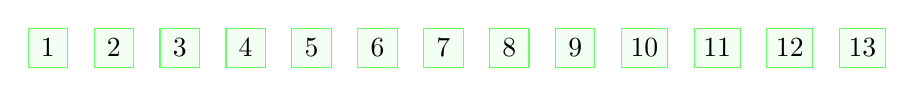
\begin{tikzpicture}[squarenode/.style={rectangle, draw=green!60, fill=green!5, thin, minimum size=5mm}]
        
        \node[squarenode] (1) {1};
        \node[squarenode] (2) [right=0.323cm of 1] {2};
        \node[squarenode] (3) [right=0.323cm of 2] {3};
        \node[squarenode] (4) [right=0.323cm of 3] {4};
        \node[squarenode] (5) [right=0.323cm of 4] {5};
        \node[squarenode] (6) [right=0.323cm of 5] {6};
        \node[squarenode] (7) [right=0.323cm of 6] {7};
        \node[squarenode] (8) [right=0.323cm of 7] {8};
        \node[squarenode] (9) [right=0.323cm of 8] {9};
        \node[squarenode] (10) [right=0.323cm of 9] {10};
        \node[squarenode] (11) [right=0.323cm of 10] {11};
        \node[squarenode] (12) [right=0.323cm of 11] {12};
        \node[squarenode] (13) [right=0.323cm of 12] {13};

        \end{tikzpicture}
    \end{tabular}
\end{center}

Just by following two simple steps, we've constructed a sorted sequence from an unordered sequence. Remember at the beginning, when I said this technique is efficient for sorting small sequences? Why is that?

\section{Analyzing Insertion Sort}

For this section, I'm going to assume some familiarity with big-O notation. If not, no worries, but I highly recommend taking a look at the document about O-notation in the root of the \verb|implementation/| directory in the repository.

\end{document}